%% Multi Figure Environment
\documentclass[12pt]{article}
\usepackage{graphicx}
\graphicspath{{Images/}} %% Path to find Image Files
\usepackage{caption} %% For using Sub-Figure and Sub-Table Environments
\usepackage{subcaption}
\usepackage[a4paper, width=150mm, top=25mm, bottom=25mm]{geometry}

\usepackage{float}
\usepackage[section]{placeins} % \FloatBarrier, it avoids floating of tables and

\begin{document}

%%Single Figure Environment

\begin{figure}[H]
    \centering
    \begin{subfigure}[b]{0.45\textwidth}
        \centering
        \includegraphics[width=\textwidth]{trac3}
        \caption{Impact of a $15^{\circ}/h$ angular rotation of collector array}
        \label{a} %% to refer use, \ref{}
    \end{subfigure}
    \hfill%% Fill Horizontal Space between two Figures
        \begin{subfigure}[b]{0.45\textwidth}
        \centering
        \includegraphics[width=\textwidth]{trac4}
        \caption{Looking down on North Pole}
        \label{a} %% to refer use, \ref{}
    \end{subfigure}
    \caption{Polar Mount for a one-axis tracker}
    \label{mfc4h1}
\end{figure}    
 
\begin{figure}[H]    
\begin{center}
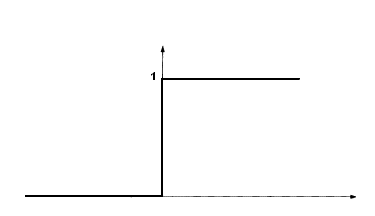
\includegraphics[width=.4\textwidth]{ANNImg4}
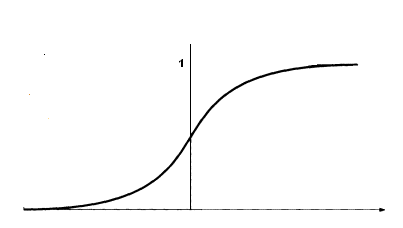
\includegraphics[width=.4\textwidth]{ANNImg5}
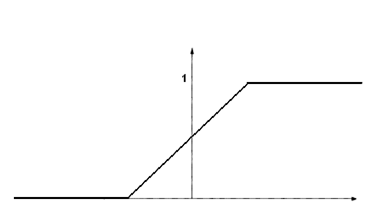
\includegraphics[width=.4\textwidth]{ANNImg6}
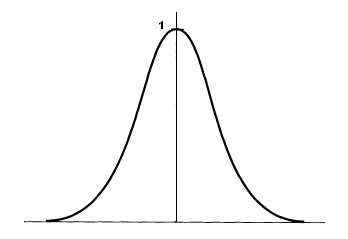
\includegraphics[width=.4\textwidth]{ANNImg7}
\end{center}
\caption{Different Activation Functions: Upper Left - Unit Step, Upper Right - Sigmoid, LowerLeft - Piecewise Linear and LowerRight - Gaussian}    
\label{ANNActFunc}
\end{figure}    
        

\end{document}